\section{Results}
\subsection{Motion captured chewing trajectories}

Figures~\ref{fig:trajectory_plot} and \ref{fig:xy-z} show a representative chewing trajectory recorded from a human subject masticating chewing gum on random sides of the mouth, using the OptiTrack motion 
capture system. The vertical displacement clearly reveals cyclic jaw movements, identifiable by recurring peaks that correspond to the opening and closing 
phases of the chewing cycle. The horizontal components (x and y) show a pattern that is qualitatively consistent with reported human data in \cite{chewing_traj}.

However, in the second half of the recording, the orientation data becomes less structured, making it difficult to extract a consistent angular pattern. Notably, 
this segment was selected for its relatively clean signal compared to other portions of the dataset. This highlights the limitations of the current motion capture 
setup in accurately capturing fine jaw dynamics.

Several factors may contribute to this inaccuracy. First, the experimental setup in the lab is optimized for larger body movements, with camera placements and 
coverage not tailored for millimeter-scale precision. Second, the marker was placed on the gnathion, a point on the skin, which does not remain rigidly coupled 
to the mandible during mastication. Skin movement introduces additional noise that likely distorts the underlying bone trajectory.

Despite these limitations, the trajectory remains sufficiently accurate to evaluate the robot's position control performance and serves as a useful initial 
benchmark.

\begin{figure}[H]
\centering
\begin{minipage}{.45\textwidth}
  \centering
  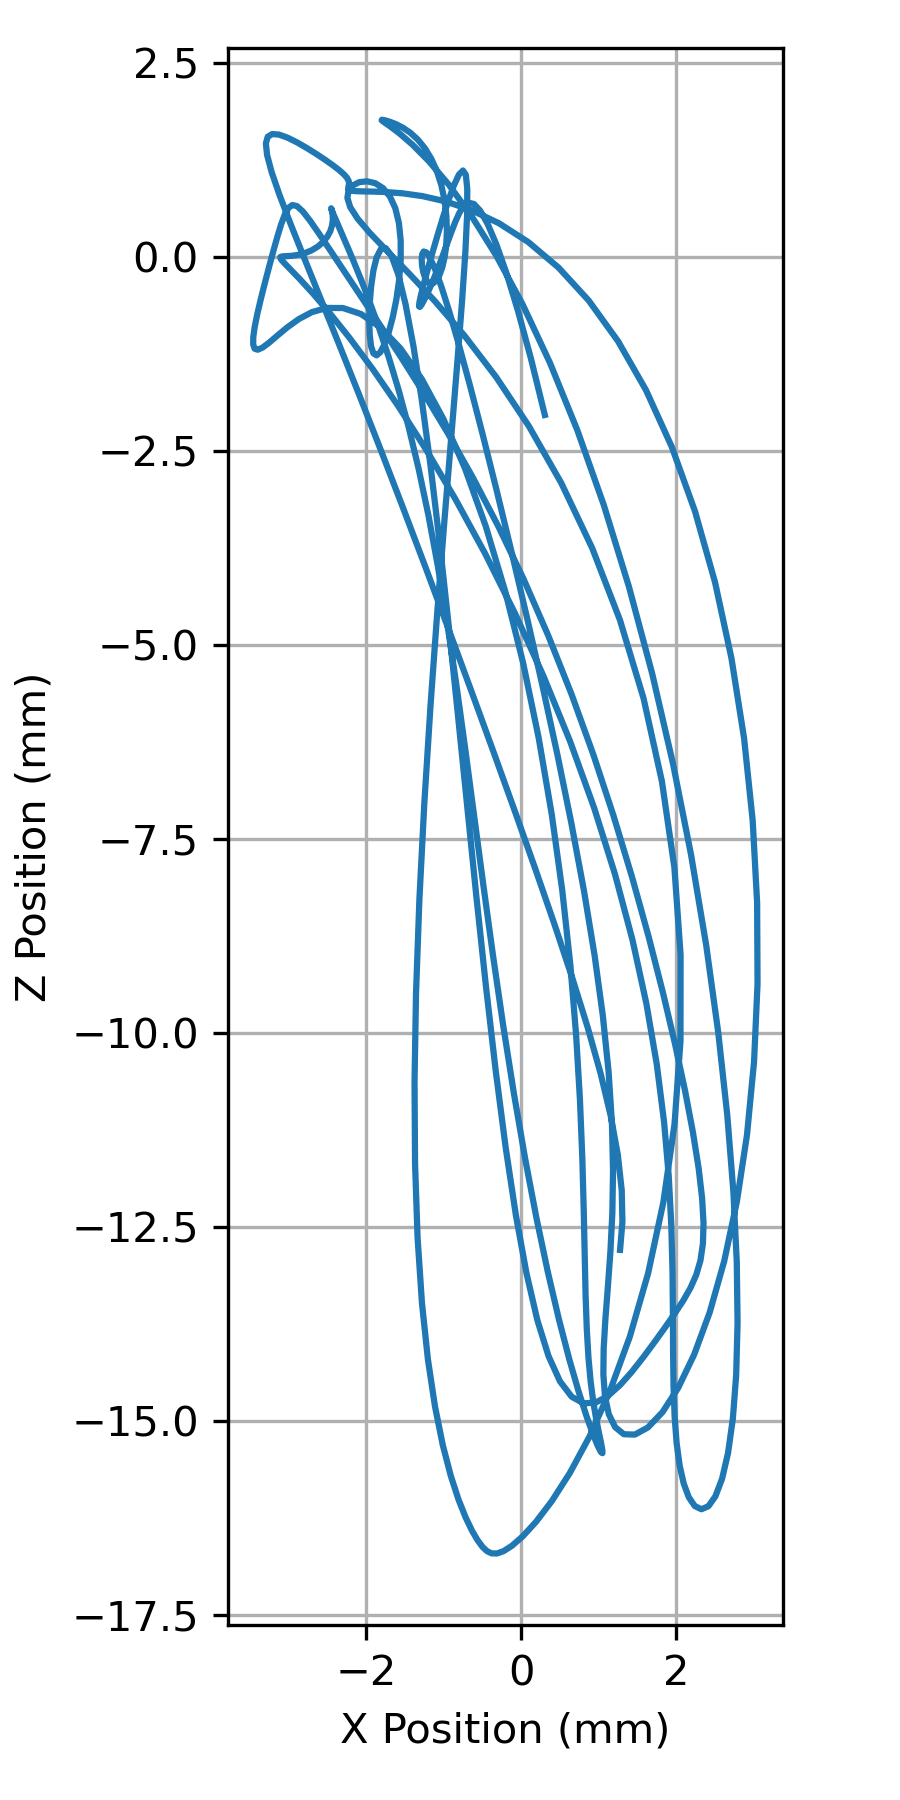
\includegraphics[height=6cm]{figures/x_vs_z_position.png}
  \subcaption{}
  \label{fig:x-z}
\end{minipage}
\begin{minipage}{.45\textwidth}
  \centering
  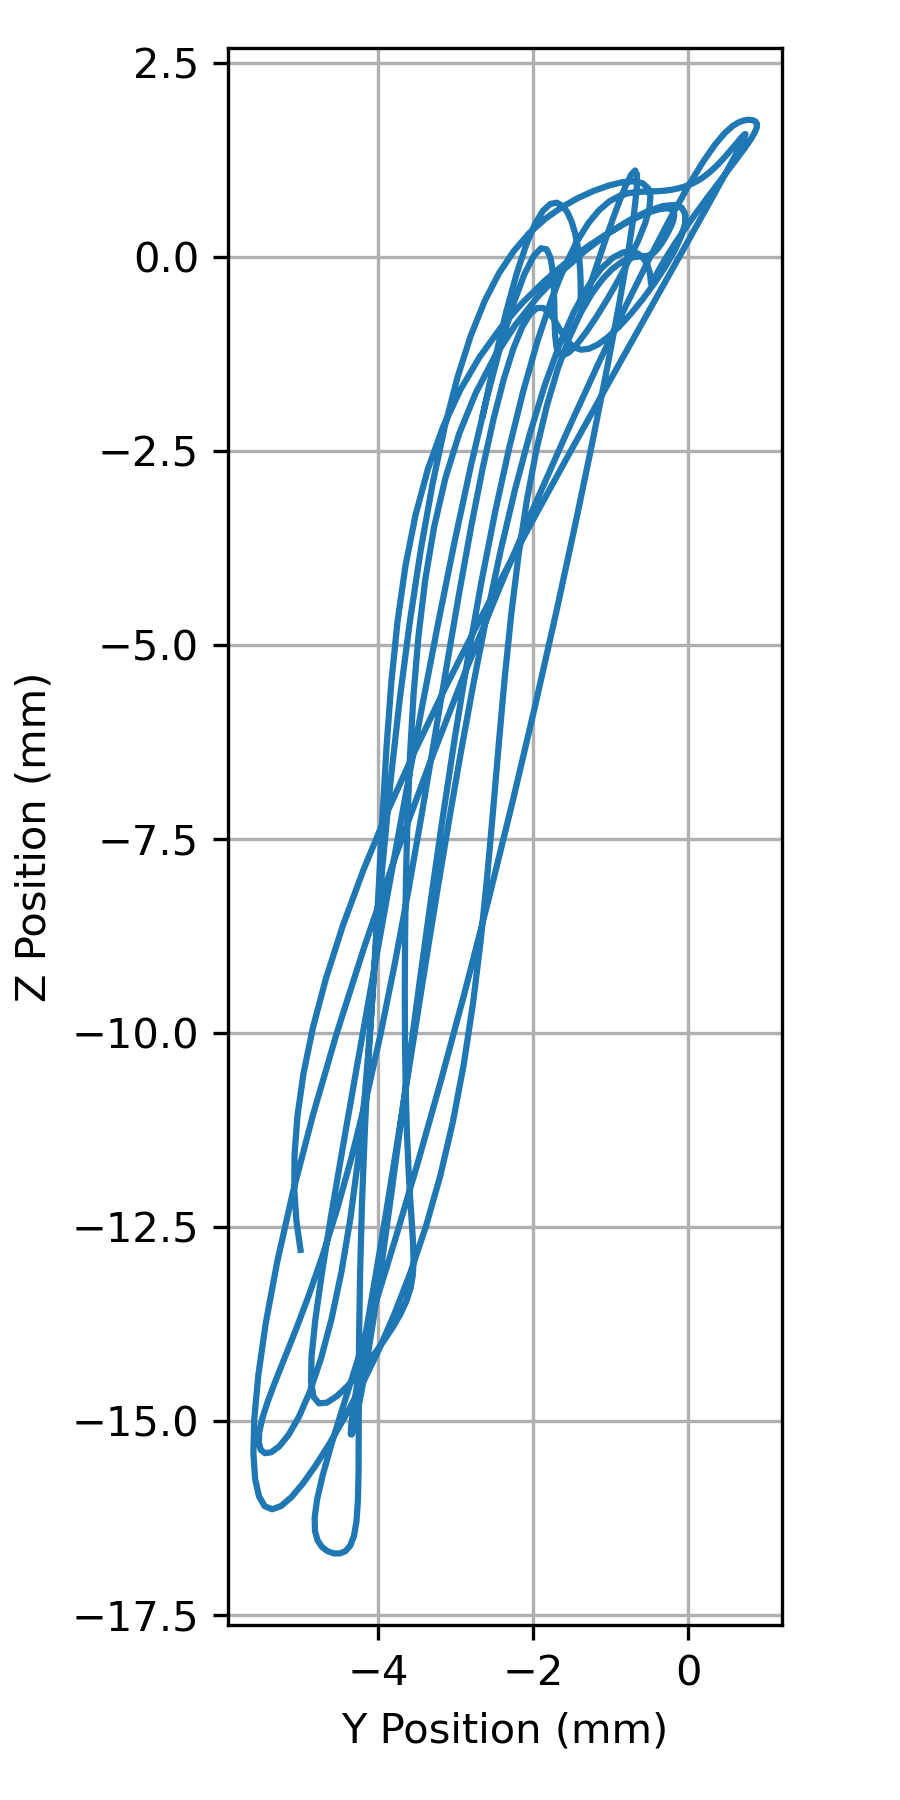
\includegraphics[height=6cm]{figures/y_vs_z_position.png}
  \subcaption{}
  \label{fig:y-z}
\end{minipage}
\caption{Position of the jaw in the x-z plane (a) and y-z plane (b).}
\label{fig:xy-z}
\end{figure}

\begin{figure}[H]
    \centering
    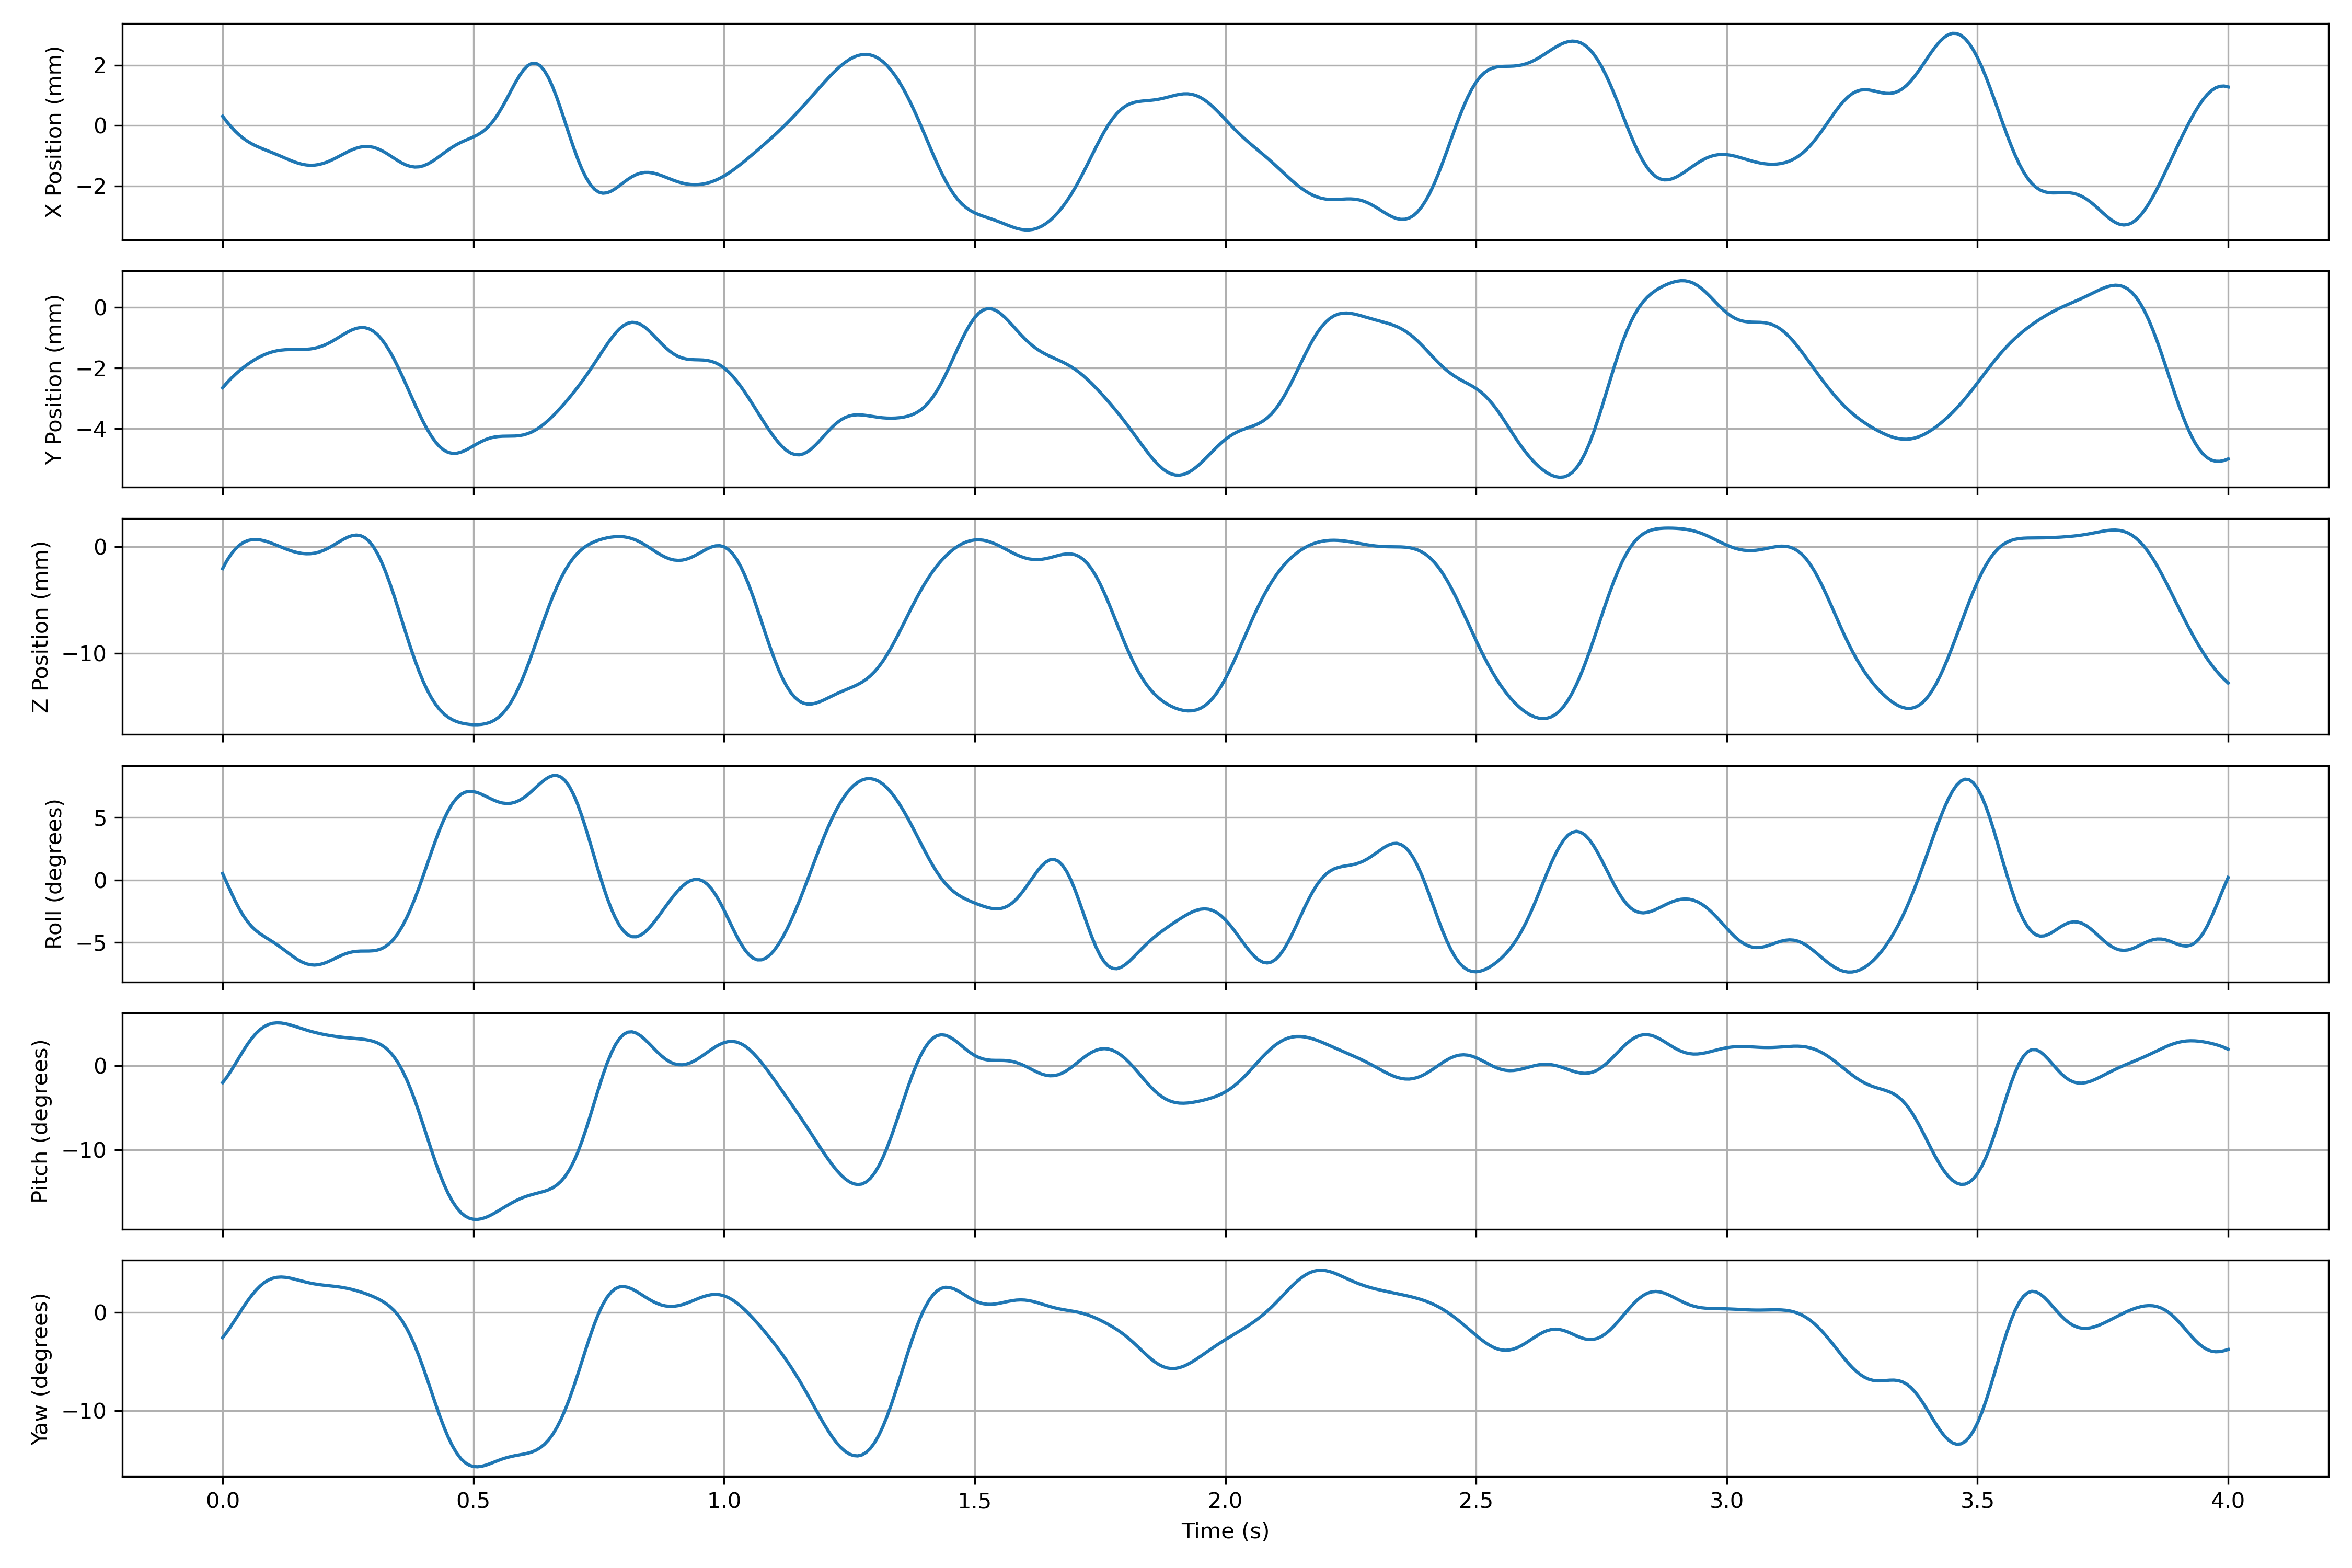
\includegraphics[width=\textwidth]{figures/trajectory_plot.png}
    \caption{Random side chewing gum mastication trajectory.}
    \label{fig:trajectory_plot}
\end{figure}

\subsection{Position control}

\paragraph{Speed and accuracy}
To evaluate the performance of the position control system, we investigated the robot's ability to track a predefined trajectory at varying speeds. 
In this context, “speed” refers to the time interval between consecutive trajectory points. While the motion capture data was recorded at 120 Hz 
(approximately every 8.3 ms), the playback was tested at longer intervals: 40 ms (25 Hz), 50 ms (20 Hz), 60 ms (16.67 Hz), 70 ms (14.29 Hz), 80 ms 
(12.5 Hz), 90 ms (11.11 Hz), and 100 ms (10 Hz).

For this test, a 10-second segment of randomly selected chewing motion was used. We recorded both the target and actual actuator lengths across all 
actuators. Figure~\ref{fig:actuator_delays_2} illustrates the tracking performance of actuator 2 at the various speeds. To quantify timing discrepancies, we 
conducted a cross-correlation analysis between the target and actual actuator lengths, providing both time delays (Figure~\ref{fig:actuator_delays_2}) 
and cross-correlation coefficients (Figure~\ref{fig:actuator_rhos_2}).

The results show that at a sampling interval of 100 ms (10 Hz), the robot tracks the trajectory well, with an average delay of ~0.7 s and 
cross-correlation coefficients exceeding 0.975. However, performance degrades significantly at higher speeds (i.e., shorter intervals), 
as reflected in both increased delays and a drop in correlation values—especially below 80 ms, where the tracking error becomes pronounced 
and key trajectory peaks are missed.

\begin{figure}[H]
    \centering
    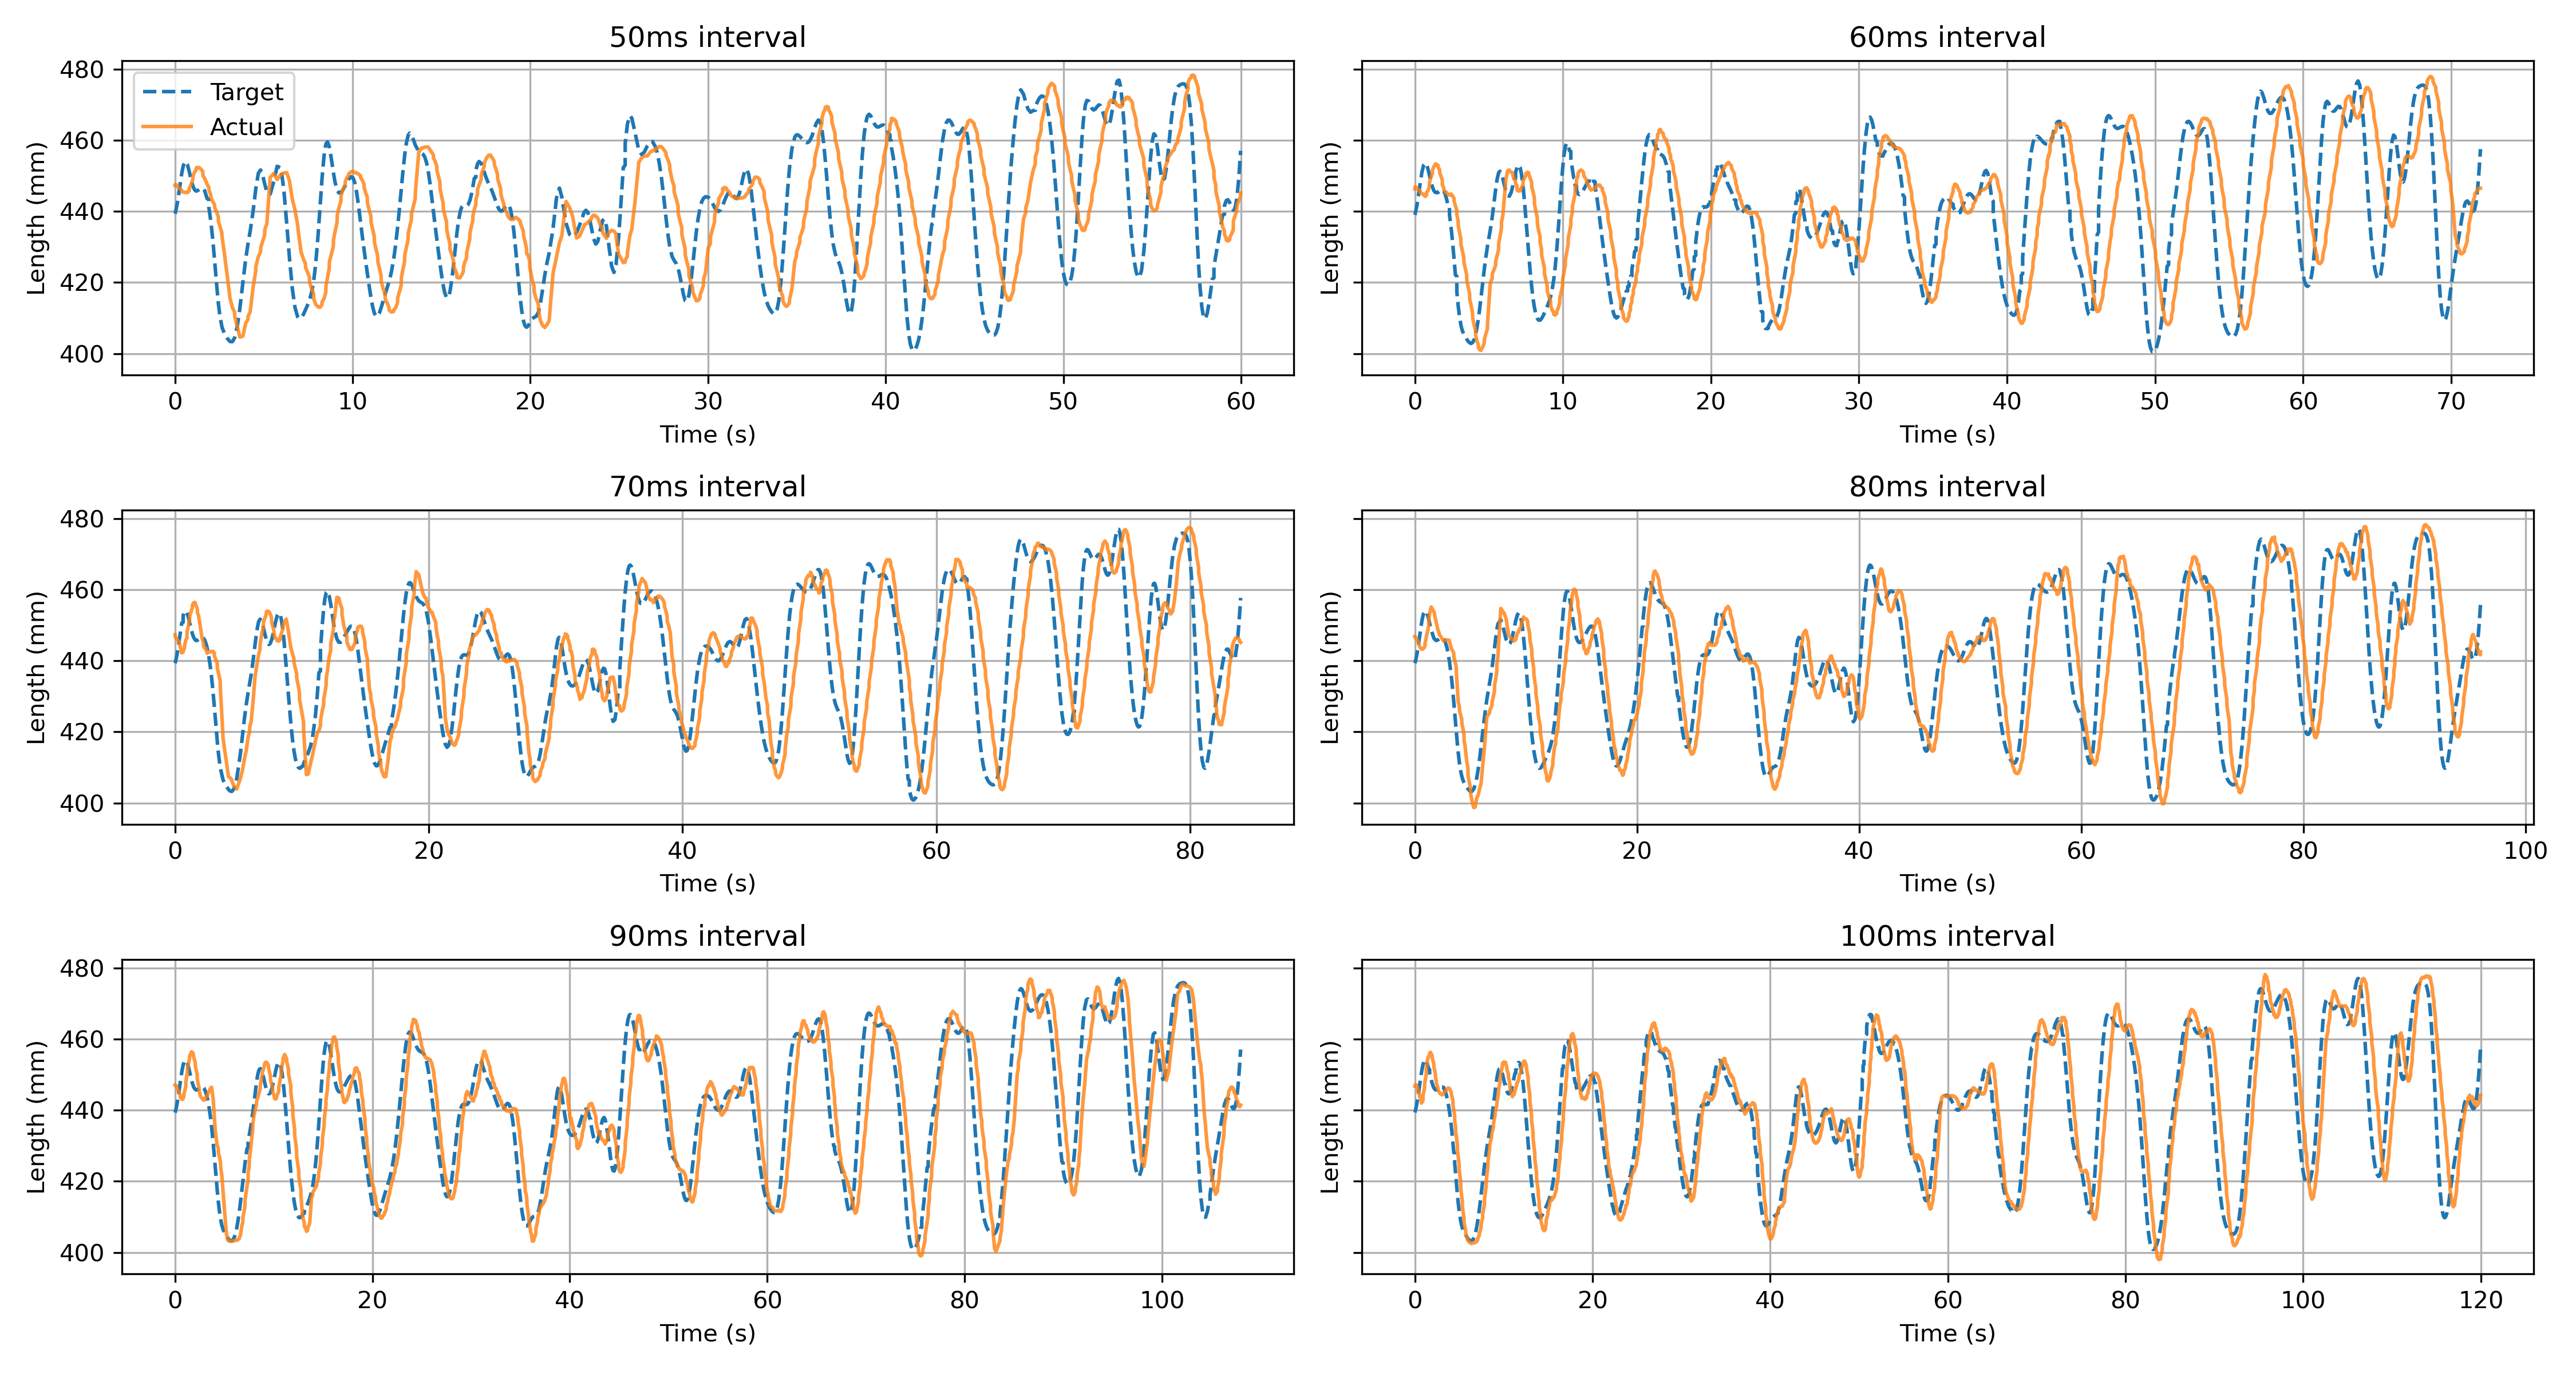
\includegraphics[width=\textwidth]{figures/actuator_2_trajectories.png}
    \caption{Performance of position control of actuator 2 across different time intervals between trajectory points.}
    \label{fig:position_control}
\end{figure}

\begin{figure}[H]
    \centering
    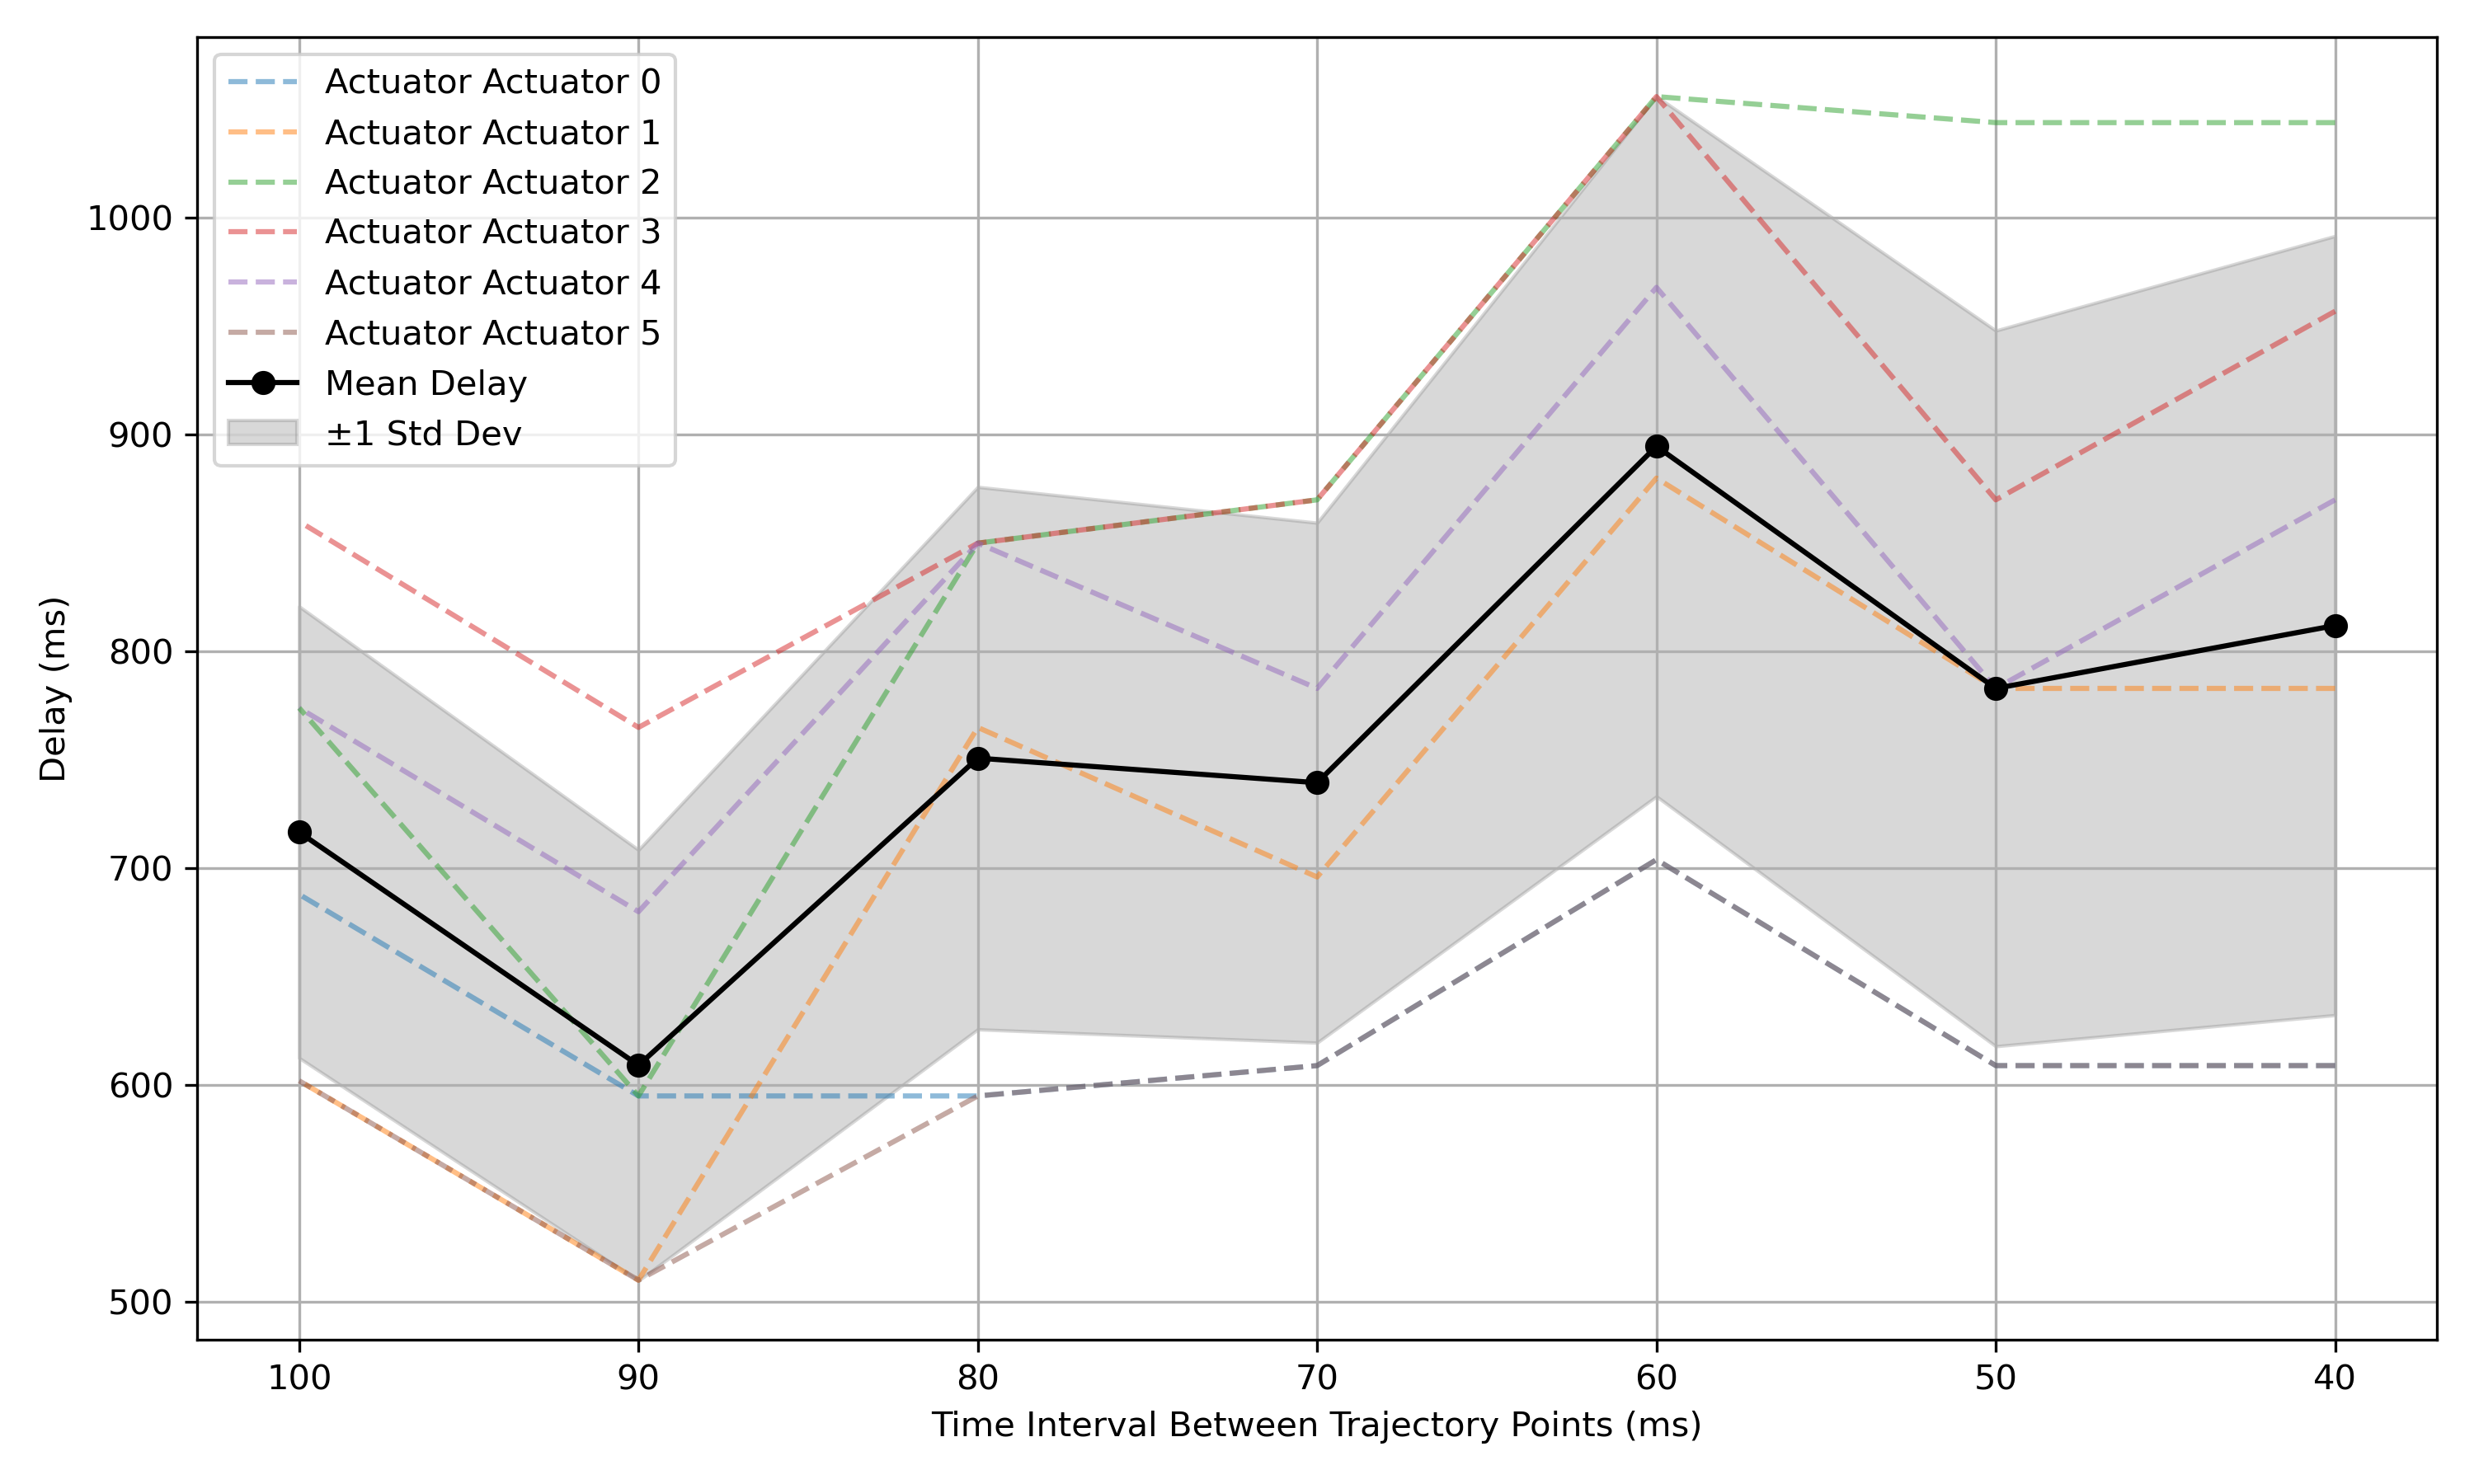
\includegraphics[width=0.9\textwidth]{figures/actuator_delays.png}
    \caption{Delays between target and actual actuator length across different time intervals.}
    \label{fig:actuator_delays_2}
\end{figure}

\begin{figure}[H]
    \centering
    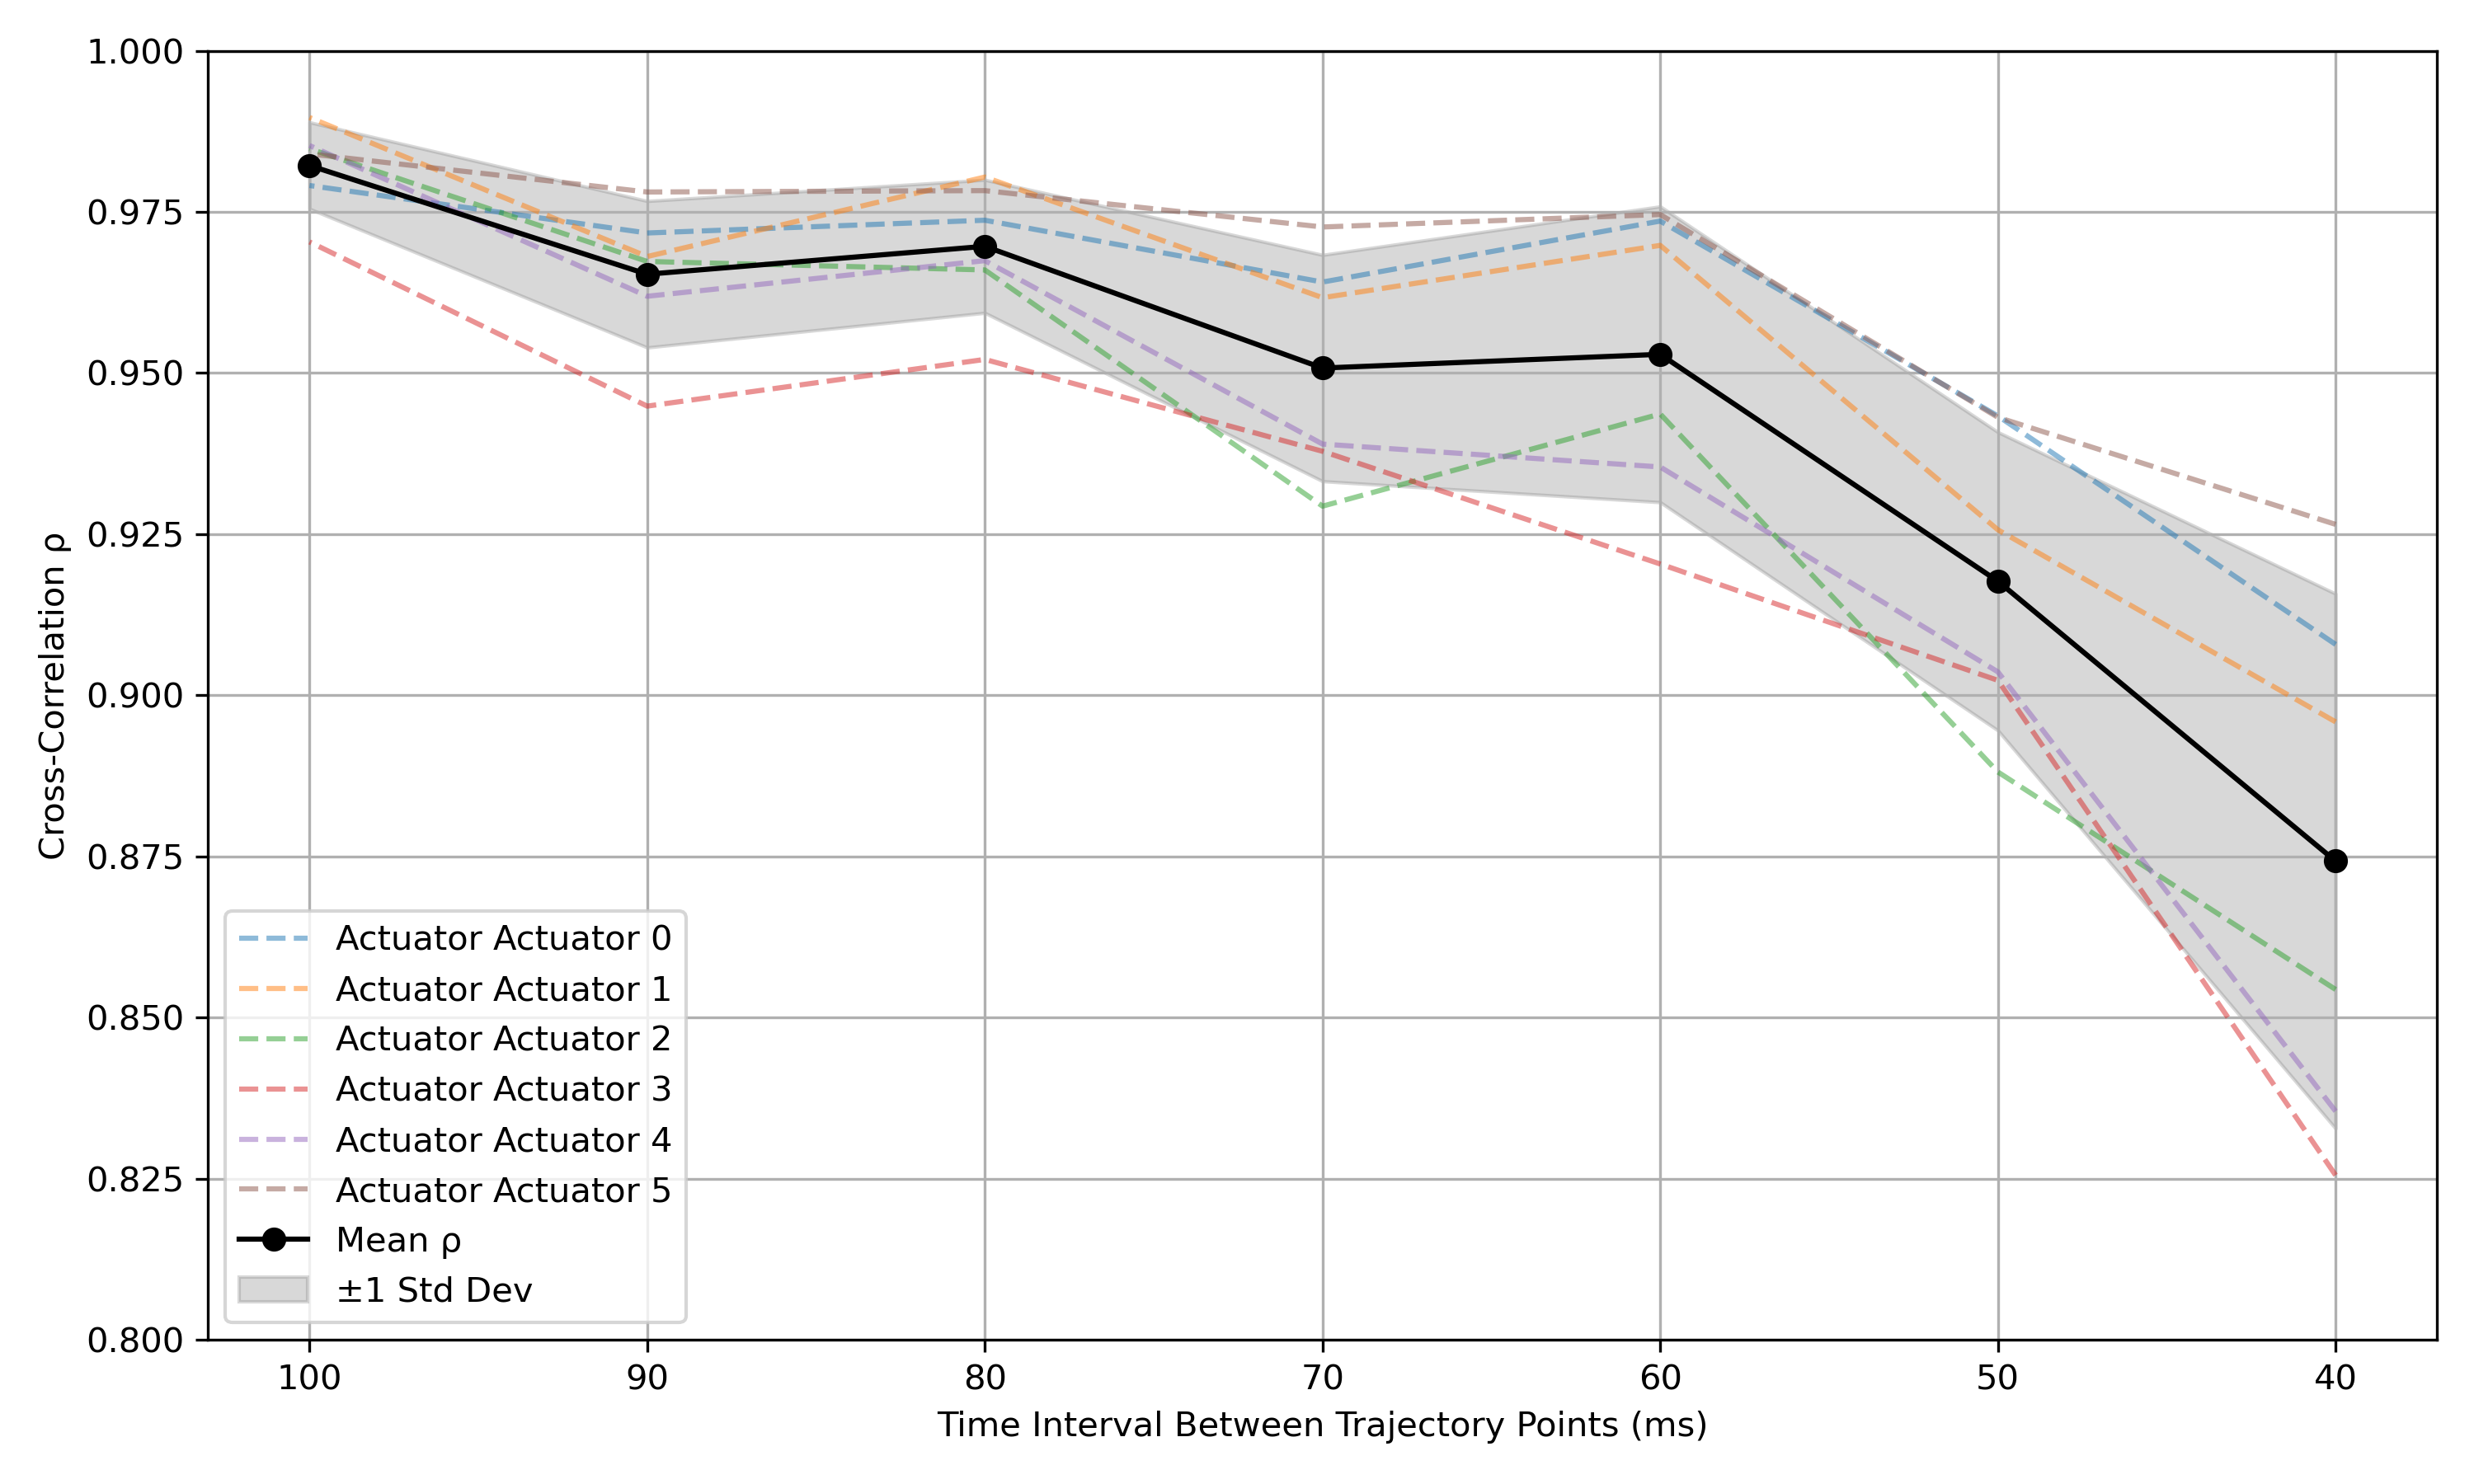
\includegraphics[width=0.9\textwidth]{figures/actuator_rhos.png}
    \caption{Cross-correlation coefficients across actuators for different time intervals.}
    \label{fig:actuator_rhos_2}
\end{figure}

\subsection{Force analysis}

\subsubsection{Maximum force}

The robot's vertical force generation capabilities were assessed using manual control mode normally used to set the robot's home position during calibration. 
The platform was driven at its highest height under active force feedback while avoiding structural failure. The upper bound of the robot's vertical force 
output was constrained by the stiffness of the upper jaw structure, which visibly bent under high vertical force. table~\ref{tab:max_force} shows the 
maximum forces recorded by the three load cells during this test, see Figure~\ref{fig:load_cells_axis}.
for the load cell positions. The results shows that most of the vertical force is applied on the back load cells, which reflects the 
anatomical load pattern during full occlusion, where the molars bear the majority of chewing forces. The total vertical force output of the robot is 
315.98 N, which is well within the average occlusal force during chewing, although below the maximum bit force from Table~\ref{tab:functional_criteria}.
%TODO: find average bite force during chewing paper
\begin{table}[H]
    \centering
    \begin{tabular}{p{4cm} p{2cm} p{2cm} p{2cm}}
        \toprule
        \textbf{Load Cell} & \textbf{$F_{z,max}$ (N)} & \textbf{$F_{y,max}$ (N)} & \textbf{$F_{x,max}$ (N)} \\
        \midrule
        Back Right Load Cell & 124.63 & x & x \\
        Back Left Load Cell & 124.63 & x & x  \\
        Front Load Cell & 66.28 & x & x  \\
        \midrule
        \textbf{Total Force} & \textbf{315.98} & x & x \\
        \bottomrule       
    \end{tabular}
    \caption{Maximal forces recorded by the load cells during the force test.}
    \label{tab:max_force}
\end{table}

%TODO: shear and protrusion forces

\subsubsection{Force feedback distribution}

To evaluate the spatial resolution of the force sensing system, we applied a simple vertical trajectory while placing a piece of gum-like material 
at three distinct positions between the teeth: back right, front, and back left. The vertical force output from each of the three load cells was 
recorded (Figure~\ref{fig:force_distribution_gum}).

The plot clearly shows three distinct peaks corresponding to the three test positions, confirming the system's capability to localize force application 
across the dental arch. Additionally, when force is applied at the back, the front load cell registers a smaller secondary response. This is consistent 
with the mechanical coupling in the mounting structure, as the front load cell is physically situated between the two rear ones.

\begin{figure}[H]
    \centering 
    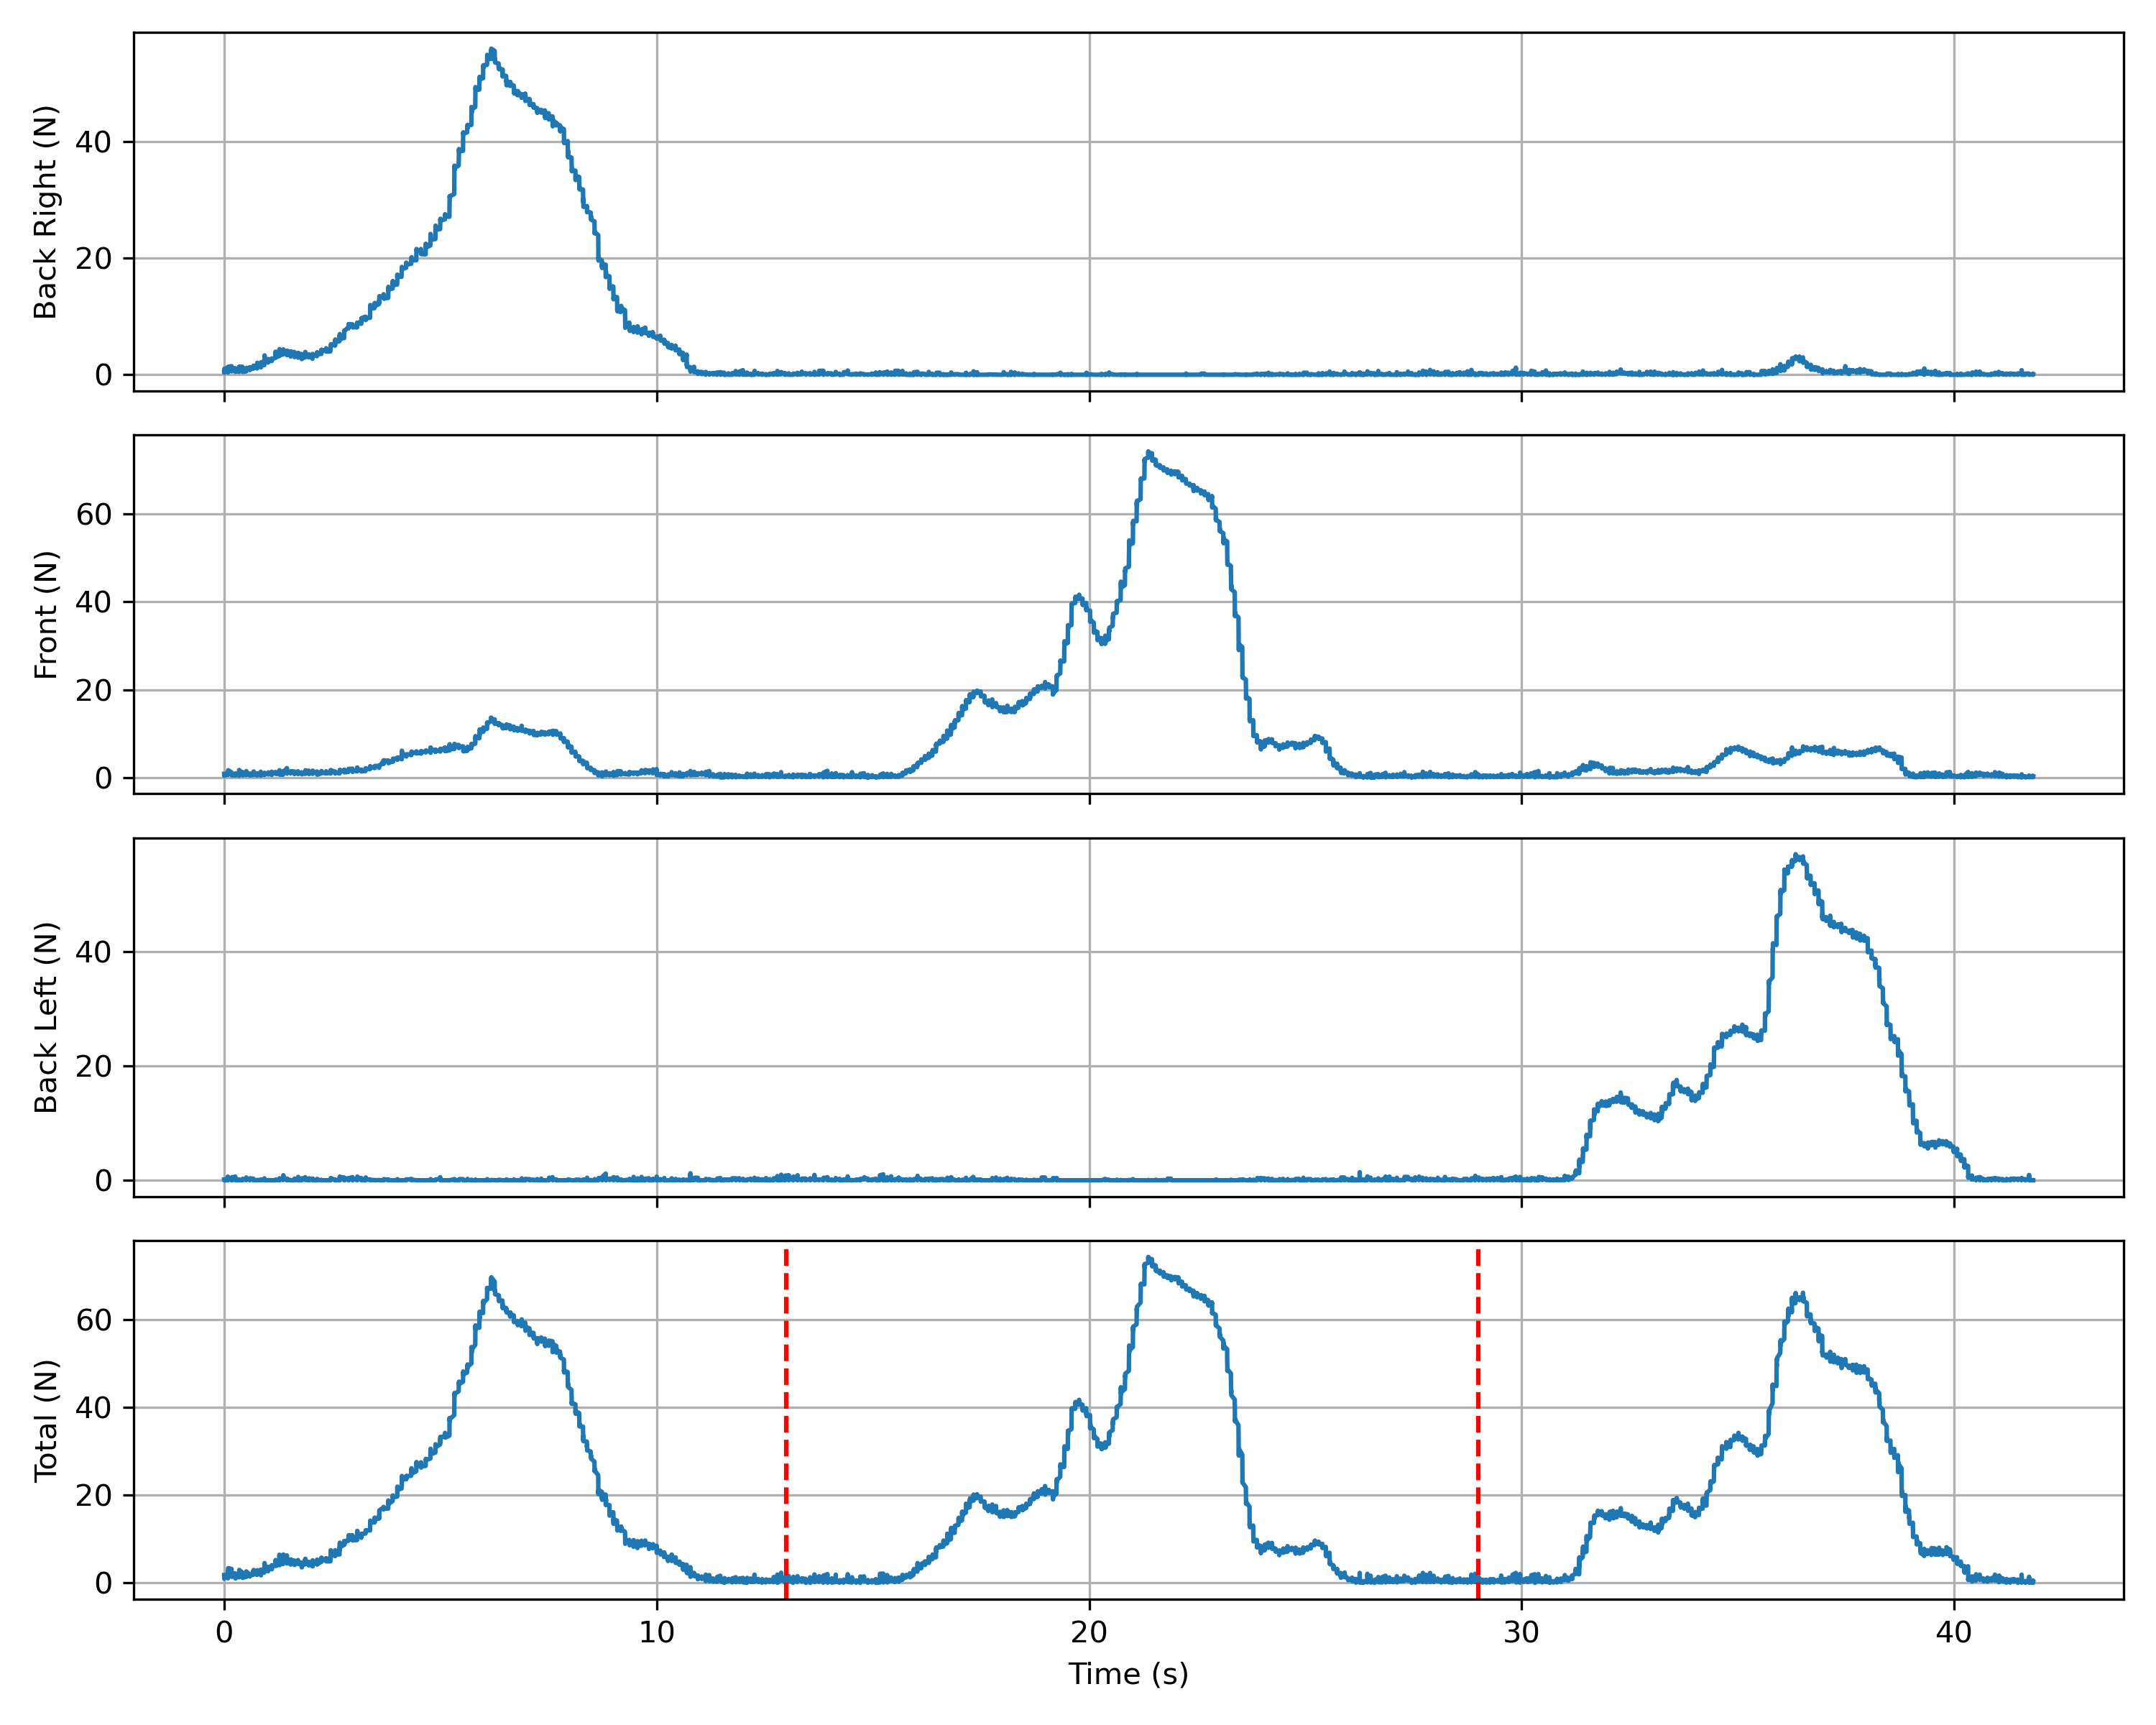
\includegraphics[width=0.8\textwidth]{figures/ForceDistributionGum.png}
    \caption{Vertical force output across three load cells during chewing with localized gum placement.  
    The red lines separate the three gum positions: back right, front, and back left.}
    \label{fig:force_distribution_gum}
\end{figure}

\subsection{Scalability and modularity}
\subsubsection{Scalability} One of the goals of the design was to create a foundation for a more complete chewing robot, like adding a tongue, saliva pumps or an esophagus. 
As described in Section~\ref{sec:mechanical_design}, the platform design and jaws subassemblies already allow for the addition of a tongue and esophagus, as well as cameras 
to monitor the chewing process. These design choices where possible thanks to the collaboration with my supervisor, Benhui Dai. Figure xxx shows a rendering of the 
robot with the future modules. As seen in Section~\ref{sec:control}, the control system is also designed to scaled to easily support additional modules, such as a tongue or esophagus. 

A central objective of this project was to design a chewing robot that could serve as a scalable platform for future extensions. As detailed in Section~\ref{sec:mechanical_design}, 
the mechanical structure of the jaws and Stewart platform has been intentionally configured to accommodate additional components such as a tongue module, saliva pumps, and an 
esophagus. Sufficient space has also been reserved for mounting internal cameras to observe the food during mastication.

These hardware design choices were made in collaboration with the project supervisor, Benhui Dai, and a first rendering of the future module tongue implemented on the lower jaw is shown in Figur~\ref{fig:tongue}.

\begin{figure}[H]
\centering
\begin{minipage}{.45\textwidth}
  \centering
  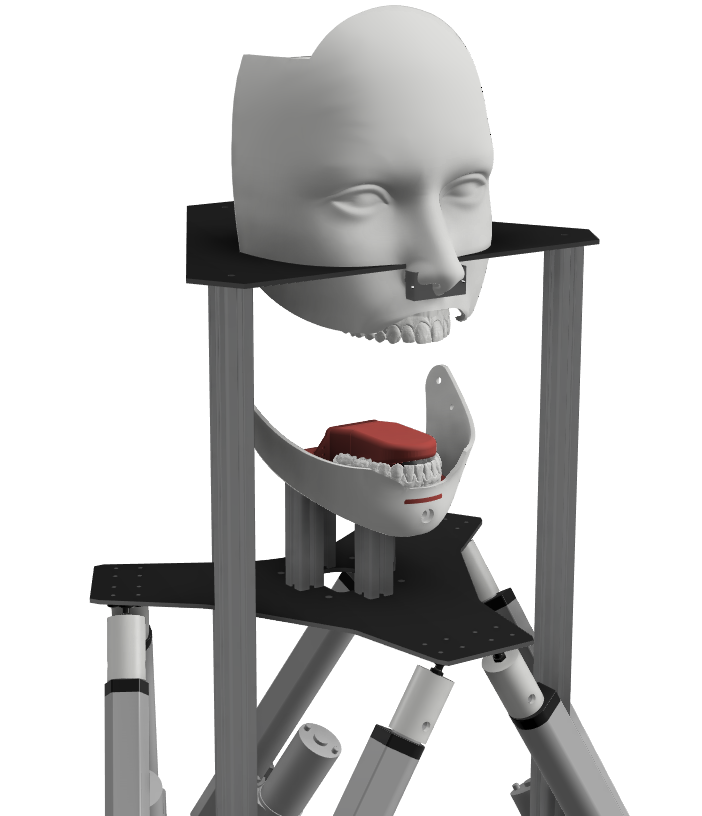
\includegraphics[height=6cm]{figures/tongue_front.png}
  \subcaption{}
  \label{fig:tongue_front}
\end{minipage}
\begin{minipage}{.45\textwidth}
  \centering
  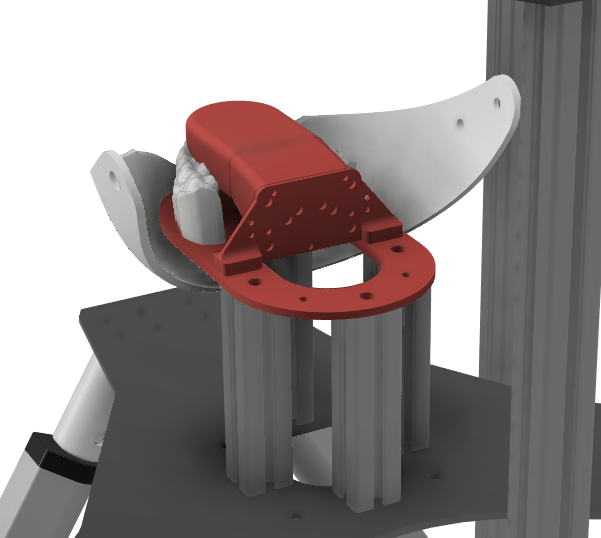
\includegraphics[height=6cm]{figures/tongue_back.png}
  \subcaption{}
  \label{fig:tongue_back}
\end{minipage}
\caption{Future tongue module rendering. (a) Front view, (b) Back view. }
\label{fig:tongue}
\end{figure}

The control system, described in Section~\ref{sec:control}, was developed with similar scalability in mind. The modular software architecture and finite-state machine 
allow for straightforward integration of new modules, including actuators, sensors, and subsystems required for tongue or saliva control.

\subsubsection{Modularity} 
The robot is designed with modularity at both the hardware and software levels. On the mechanical side, key components such as the mandibular and maxillary teeth are mounted using 
replaceable acrylic adaptors, enabling rapid swaps for testing different dentitions. This feature is particularly relevant for simulating conditions such as orthodontic treatments, 
dental implants, or age-related tooth wear.

**TODO: Example of new teeth?**

On the software side, adaptation to new dental configurations only requires updating the initial platform position to achieve full occlusion. New chewing trajectories can be added to 
the micro-SD card and executed without code modification, making the robot well-suited for testing diverse experimental scenarios and clinical applications.


